\documentclass[12pt]{report}

% ================== BASIC PACKAGES ==================
\usepackage[utf8]{inputenc}
\usepackage[T1]{fontenc}
\usepackage[english]{babel}
\usepackage{setspace}
\usepackage{geometry}
\usepackage{graphicx}
\usepackage{float}
\usepackage{booktabs}
\usepackage{hyperref}
\usepackage{tikz}
\usetikzlibrary{positioning}
\usepackage{float}

% ================== PAGE SETTINGS ==================
\geometry{a4paper, margin=1in}
\onehalfspacing

\begin{document}

% ================== TITLE PAGE ==================
\begin{titlepage}
    \centering
    
    {\Large \textbf{Titanic: Machine Learning from Disaster} \par}
    \vspace{0.5cm}
    {\large \textbf{System Analysis Project} \par}
    \vspace{3cm}
    
    {\large 
    Julián Carvajal Garnica \\ 
    20242020024 \\[0.5cm]
    Andrés Mauricio Cepeda Villanueva \\
    20242020010 \\[0.5cm]
    Jhonatan David Moreno Barragán \\
    20201020094 \\[0.5cm]
    Andrés Camilo Ramos Rojas \\
    20242020005
    }
    
    \vfill
    
    School of Engineering, Universidad Distrital Francisco José de Caldas \\
    System Analysis Course \\
    Teacher: Carlos Andrés Sierra \\
    Bogotá D.C. \\
    2025
    
\end{titlepage}

% ================== PART 3 ==================
\chapter*{Part 3 of the System Analysis Project}

\section*{1. Review and Refine System Architecture}

Based on the high-level architecture defined in Part 2, this section refines the design to incorporate robust engineering principles, as requested in Workshop 3. The goal is to evolve our predictive system from a prototype to a sustainable solution, explicitly addressing reliability, scalability, and maintainability.

\subsection*{1.1 Refinement of Robust Design Principles}

The original architecture established a modular flow. We now refine this with an explicit focus on robustness:

\begin{itemize}
    \item \textbf{Modularity and Maintainability (CMMI):} We are taking modularity a step further. Each component (Ingestion, Preprocessing, Modeling, Evaluation) [cite: 96-100] will be designed as a containerized microservice (e.g., using Docker). This not only reinforces modularity but also aligns with \textbf{CMMI} principles by allowing independent configuration management and facilitating maintainability, as one component can be updated without destabilizing the entire system.

    \item \textbf{Scalability:} The scalability NFR will be addressed through the orchestration of these containers (e.g., with Kubernetes). Specifically, the \textit{Modeling Layer} and \textit{Deployment Layer} will be able to scale horizontally. If the demand for Titanic predictions increases, we can dynamically launch more instances of the \textit{Deployment} service.

    \item \textbf{Fault-Tolerance:} This is a critical refinement.
    \begin{itemize}
        \item \textbf{Data Ingestion:} A message queue (e.g., RabbitMQ or Kafka) will be implemented between the ingestion and preprocessing layers. If the \textit{Preprocessing Layer} fails, the raw Kaggle data is not lost; it waits in the queue, ensuring \textbf{reliability}.
        \item \textbf{Deployment:} A load balancer will be used to distribute prediction requests among multiple model replicas. If one replica fails, traffic is automatically rerouted to healthy ones.
        \item \textbf{Feedback Loop:} The \textit{Feedback Layer} will monitor model health. If the error rate (an indicator of chaos) exceeds a threshold, the system can automatically roll back to a previously stable model version, ensuring \textbf{homeostasis}.
    \end{itemize}
\end{itemize}

\subsection*{1.2 Components and their Support for Quality (ISO 9000)}

Following the process management principle of \textbf{ISO 9000}, we define how each component ensures system quality and reliability:

\begin{itemize}
    \item \textbf{Data Ingestion Layer:}
    \begin{itemize}
        \item \textit{Quality:} Implements data validation schemas (e.g., Pydantic) to ensure incoming data meets the expected format (data types, ranges).
        \item \textit{Reliability:} Uses retries and the message queue (see above) to handle network failures or Kaggle service downtime.
    \end{itemize}
    
    \item \textbf{Preprocessing Layer:}
    \begin{itemize}
        \item \textit{Quality:} Versioning of preprocessing artifacts (e.g., Scikit-learn scalers or encoders) is implemented. Each trained model will be linked to the exact version of the preprocessing pipeline it used, ensuring \textbf{transparency} and reproducibility.
    \end{itemize}
    
    \item \textbf{Modeling \& Evaluation Layer:}
    \begin{itemize}
        \item \textit{Quality:} We apply a \textit{Six Sigma} approach to "defect reduction" (prediction errors). The \textit{Evaluation Layer} will not only measure accuracy but also use SHAP and LIME to analyze the \textit{root cause} of errors and bias, aligning with the "Analyze" phase of DMAIC.
    \end{itemize}
    
    \item \textbf{Deployment \& Feedback Layer:}
    \begin{itemize}
        \item \textit{Reliability:} Implements "Canary" deployments. A new model version is first released to a small percentage of users. The \textit{Feedback Layer} monitors its real-time performance. If stable, it is rolled out to everyone; if it fails, it is rolled back without affecting the majority of users.
    \end{itemize}
\end{itemize}


% ----------------------------------------------------------
\section*{2. Quality and Risk Analysis}

Designing a robust system for the Titanic Kaggle Competition requires aligning quality management principles with systems thinking. The goal is to ensure reliability, scalability, maintainability, and adaptability, while managing uncertainty and sensitivity derived from the system’s inherent complexity.

% ----------------------------------------------------------
\subsection*{2.1 Quality Foundations}

The system follows international quality frameworks to guarantee structural integrity and continuous improvement:

\begin{itemize}
    \item \textbf{ISO 9000 (Quality Management):} Ensures customer-focused design, process consistency, and continuous improvement throughout the system lifecycle.
    \item \textbf{CMMI (Capability Maturity Model Integration):} Guides process optimization and project control, establishing measurable quality benchmarks.
    \item \textbf{Six Sigma:} Provides statistical discipline for minimizing variation and data-driven decision-making, aligning with the need to control model sensitivity and randomness.
\end{itemize}

Each guideline reinforces systemic robustness by treating errors not as isolated faults but as signals for feedback, self-correction, and adaptation—echoing the principles of homeostasis and self-regulation in complex systems.

% ----------------------------------------------------------
\subsection*{2.2 Risk and Failure Analysis}

\begin{table}[H]
\centering
\resizebox{\textwidth}{!}{
\begin{tabular}{|p{3.5cm}|p{5.5cm}|p{6cm}|p{5cm}|}
\hline
\textbf{Risk / Failure Point} & \textbf{Description} & \textbf{Mitigation Strategy} & \textbf{Monitoring Mechanism} \\ \hline
\textbf{1. Data Quality and Loss} & Missing, biased, or corrupted data during preprocessing may distort model predictions and compromise system reliability. & Implement redundancy in data ingestion (dual pipelines), use validation scripts for integrity checks, and store datasets in version-controlled repositories. & Scheduled data audits, automatic validation logs, and alerts for anomalies in input distributions. \\ \hline
\textbf{2. Model Overfitting and Sensitivity} & The system may become overly dependent on specific features, leading to poor generalization and chaotic behavior under new data. & Apply regularization, cross-validation, and ensemble methods to reduce variance; introduce stochastic perturbations to simulate uncertainty and test robustness. & Periodic retraining with fresh data; sensitivity analysis reports visualizing feature influence. \\ \hline
\textbf{3. System Downtime or Integration Failure} & Interruption in deployment pipelines or feedback loops can halt adaptation and degrade performance. & Design a modular architecture with fault tolerance and fallback modes; implement containerized environments (Docker) for isolation and recovery. & Continuous integration (CI/CD) logs, health-check endpoints, and uptime dashboards. \\ \hline
\textbf{4. Security and Data Confidentiality} & Unprotected interfaces or leaks could expose passenger data or system configurations. & Adopt ISO 27001 guidelines—data encryption, access control, and secure API endpoints. & Automated penetration testing and incident response monitoring. \\ \hline
\textbf{5. Concept Drift and Environmental Change} & The statistical relationships in data may evolve over time, producing degraded accuracy. & Integrate dynamic feedback and retraining loops; trigger model updates based on performance thresholds. & Drift detection algorithms comparing recent vs. baseline accuracy metrics. \\ \hline
\end{tabular}
}
\caption{Risk and Failure Analysis with Mitigation Strategies}
\end{table}


% ----------------------------------------------------------
\subsection*{2.3 Systemic Integration of Quality and Risk Control}

This system applies quality assurance as a living process—not a static checklist. Through continuous feedback and adaptive response, it mirrors the homeostatic regulation seen in natural systems: deviations are sensed, processed, and corrected to restore equilibrium.

Quality and risk management act as dual forces in systemic harmony:
\begin{itemize}
    \item \textbf{Quality guidelines} create structure and predictability (deterministic behavior).
    \item \textbf{Risk management} embraces variability and chaos, converting it into controlled adaptability.
\end{itemize}

In practice, each identified risk becomes a node in a feedback network, transforming vulnerabilities into learning opportunities. The balance between control (stability) and flexibility (adaptability) ensures that the Titanic predictive system remains resilient, sustainable, and intelligent in the face of uncertainty.

% ----------------------------------------------------------
\section*{3. Project Management Plan}

The project management plan outlines how the team will manage tasks, track progress, and guarantee that the system design and implementation develop in a systematic and regulated way. This strategy adheres to fundamental project management concepts, integrating role specification, milestone scheduling, and agile organizational tools

\subsection*{3.1 Team Roles and Responsibilities}

\begin{table}[H]
\centering
\begin{tabular}{|p{5cm}|p{9cm}|}
\hline
\textbf{Role} & \textbf{Responsibilities} \\
\hline
\textbf{Project Manager (Andrés Camilo Ramos)} & Oversees the project timeline, assigns tasks, and ensures coordination between members. \\
\hline
\textbf{System Analyst (Julián Carvajal)} & Reviews system requirements, maintains consistency with previous workshops, and validates design improvements. \\
\hline
\textbf{Data Engineer (Jhonatan Moreno)} & Manages data ingestion, cleaning, and transformation processes, ensuring dataset integrity and reliability. \\
\hline
\textbf{Machine Learning Developer (Andrés Cepeda)} & Implements and tunes machine learning models, evaluates performance, and applies optimization strategies. \\
\hline
\textbf{QA Tester (All Members)} & Verifies outputs, checks accuracy of predictions, and documents bugs or inconsistencies during testing. \\
\hline
\end{tabular}
\caption{Team Roles and Responsibilities}
\label{tab:team_roles}
\end{table}

\subsection*{3.2 Key milestones and Deliverables}

\begin{table}[H]
\centering
\begin{tabular}{|p{4cm}|p{8.5cm}|p{3cm}|}
\hline
\textbf{Milestone} & \textbf{Description} & \textbf{Deadline} \\
\hline
\textbf{System Refinement} & Incorporate robust design principles (modularity, fault-tolerance, scalability) into the existing architecture. & November 16, 2025 \\
\hline
\textbf{Risk and Quality Analysis} & Identify potential system risks and define mitigation strategies aligned with ISO 9000 and CMMI principles. & November 19, 2025 \\
\hline
\textbf{Prototype Update} & Integrate refined modules and apply monitoring mechanisms to handle sensitivity and chaotic data behavior. & November 23, 2025 \\
\hline
\textbf{Final Documentation} & Compile the complete Workshop 3 report (architecture, risks, project plan, and improvements) and perform final peer review. & November 28, 2025 \\
\hline
\end{tabular}
\caption{Updated Project Milestones and Deadlines}
\label{tab:project_milestones}
\end{table}

\subsubsection*{3.3 Methodology and Tools}

The project adopts an \textbf{Agile-oriented methodology} supported by a \textbf{Kanban workflow} to ensure flexibility, collaboration, and continuous improvement throughout development. This approach divides the process into small, manageable tasks that can be completed and reviewed incrementally, maintaining full visibility of progress and priorities.

From a technical perspective, the workflow is structured as follows:

\begin{itemize}
    \item \textbf{Data Acquisition and Cleaning:} Import and preprocess the \textit{train.csv} and \textit{test.csv} datasets using \textbf{Pandas} and \textbf{NumPy}, handling missing values and ensuring data consistency.
    
    \item \textbf{Feature Engineering:} Transform categorical variables such as \textit{Sex}, \textit{Pclass}, \textit{SibSp}, and \textit{Parch} into numerical form and create new relevant attributes to improve model performance.
    
    \item \textbf{Model Training and Evaluation:} Implement machine learning algorithms from \textbf{Scikit-learn}, such as \textit{Decision Tree} and \textit{Random Forest}, to predict survival outcomes. Model performance will be evaluated using metrics like accuracy and F1-score.
    
    \item \textbf{Prediction and Submission:} Generate a \textit{submission.csv} file with the model’s predictions and validate the results within the Kaggle competition environment.
\end{itemize}

For project coordination, a \textbf{Kanban board} (implemented in \textbf{Trello} or \textbf{GitHub Projects}) will be used to organize tasks in three main columns:

\begin{itemize}
    \item \textbf{To Do:} Tasks that are planned but not yet started.
    \item \textbf{In Progress:} Tasks currently being worked on.
    \item \textbf{Completed:} Finished tasks that have been reviewed and verified.
\end{itemize}

This methodology and toolset allow for effective task distribution, smooth team collaboration, and clear progress tracking, ensuring that all project components are developed in a structured and iterative manner.

\subsection *{3.4 Timeline and Workflow Diagram}

\begin{figure}[H]
\centering
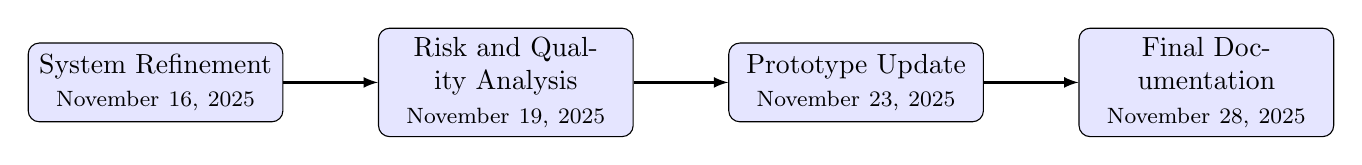
\begin{tikzpicture}[
    node distance=1.8cm and 1.2cm,
    milestone/.style={rectangle, rounded corners, draw=black, fill=blue!10, text width=3cm, align=center, minimum height=1cm},
    arrow/.style={-latex, thick}
]

% Nodes
\node[milestone] (refine) {System Refinement \\ \footnotesize November 16, 2025};
\node[milestone, right=of refine] (risk) {Risk and Quality Analysis \\ \footnotesize November 19, 2025};
\node[milestone, right=of risk] (prototype) {Prototype Update \\ \footnotesize November 23, 2025};
\node[milestone, right=of prototype] (final) {Final Documentation \\ \footnotesize November 28, 2025};

% Arrows
\draw[arrow] (refine) -- (risk);
\draw[arrow] (risk) -- (prototype);
\draw[arrow] (prototype) -- (final);

\end{tikzpicture}
\caption{Project Workflow and Timeline}
\label{fig:project_timeline}
\end{figure}


% ----------------------------------------------------------
\section*{4. Incremental Improvements}
Based on the brief feedback from previous workshops, the system design and management plan have evolved significantly. The initial focus was reassessed to concentrate on the data provided by the Kaggle competition, at a problem to solve, leading to a more robust and formalized approach. The following enhancements were implemented in response:

\begin{itemize}
    \item \textbf{Integration of Formal Quality and Risk Management:} To improve robustness, maintainability, and reliability, the system design now incorporates international quality frameworks. This includes \textbf{ISO 9000} for process consistency, \textbf{CMMI} for process optimization, and \textbf{Six Sigma} to minimize variation. This structured approach provides a formal way to manage identified risks, such as \textbf{Data Quality} and \textbf{Model Overfitting}, converting vulnerabilities into learning opportunities].

    \item \textbf{Formalized Project Management Methodology:} The project's management has been structured to ensure development occurs in a systematic and regulated manner. An \textbf{Agile-oriented methodology} supported by a Kanban workflow was adopted to enhance flexibility and collaboration. This evolution includes a clear definition of team roles, such as Project Manager and System Analyst, and a precise schedule of milestones and deliverables, ensuring clear progress tracking and that all project components are developed iteratively.
\end{itemize}
\end{document}
